\section{I/O Einheit}
\index{I/O Einheit}
\label{sec:IO-Einheit}

Die I/O-Architektur der UMach Maschine ist am sogenannten \glqq Port-Mapped
I/O\grqq\ angelehnt\footnote{Als Gegenstück von \glqq Memory Mapped I/O\grqq.}.


Die I/O-Einheit der UMach Maschine besteht aus einer Reihe von Eingangs- und
Ausgangschnittstellen, auch Ports\index{Port}\index{UMach!Port} genannt. An
diesen Ports können verschiedene physikalische Geräte angeschlossen werden, die
die entsprechenden Daten generieren bzw. verarbeiten können. Siehe dazu auch die
Abbildung \ref{fig:umach-aufbau} auf der Seite \pageref{fig:umach-aufbau}.

Die I/O Ports sind in zwei Kategorien unterteilt: Eingabeports und
Ausgabeports. Von der Bauart und Struktur her, gibt es innerhalb der jeweiligen
Kategorie keine Unterschiede zwischen Ports. Sie werden lediglich anhand deren
Nummern identifiziert.

Die Eingabe- und Ausgabefunktionen können durch bestimmten Instruktionen
gesteuert werden (siehe auch den Abschnitt \ref{sec:IO-Instruktionen}, auf der
Seite \pageref{sec:IO-Instruktionen}).


\subsection{Eingabeports}

Diese Ports sind derzeit noch nicht spezifiziert.



\subsection{Ausgabeports}

\begin{figure}[htp]
 \centering
 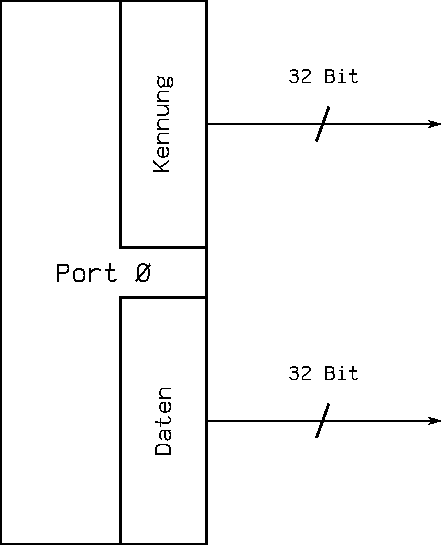
\includegraphics{./img/UMach-IOPort.pdf}
 \caption{I/O Ausgangsport}
 \label{fig:IOPort}
\end{figure}












